\documentclass[12pt,a4paper]{article}
% The following LaTeX packages must be installed on your machine: amsmath, authblk, bm, booktabs, caption, dcolumn, fancyhdr, geometry, graphicx, hyperref, latexsym, natbib
\input{183.dat}
\usepackage{gensymb}
\usepackage{amsthm}
\usepackage{float}
\usepackage{siunitx}
\usepackage{amssymb}
\usepackage{float}
\usepackage{enumerate}
\usepackage{listings}
\usepackage{mathtools}
\PassOptionsToPackage{hyphens}{url}\usepackage{hyperref}
\usepackage[none]{hyphenat}
\usepackage{physics}
\newcommand\ddfrac[2]{\frac{\displaystyle #1}{\displaystyle #2}}
%\renewcommand{\familydefault}{\sfdefault}


\begin{document}

\setcounter{page}{1}

\section*{LE3 Problem 3}
\bigskip

The describing function calculated from Problem 2 was

\begin{equation}
	N(M,\omega) = -\frac{4jA}{\pi M} \label{eq:N}
\end{equation}

And we cascade this with a process

\begin{equation}
	G(s) = \frac{5}{s(1+s)^2} \label{eq:G}
\end{equation}

\begin{enumerate}[a)]

\item \textbf{Calculation for $\omega$}

We express $G(s)$ as a frequency response

\begin{align}
	G(j\omega) &= \frac{5}{j\omega (1 + j\omega)^2} \\
	&= \frac{5}{j\omega (1 + 2j\omega - \omega^2)} \\
	&= \frac{5}{-2\omega^2 + j(\omega - \omega^3)} \\
	&= \frac{5}{-2\omega^2 + j(\omega - \omega^3)} \cdot \frac{-2\omega^2 + j(\omega - \omega^3)}{-2\omega^2 + j(\omega - \omega^3)} \\
	&= \frac{-10\omega^2 + 5j(\omega - \omega^3)}{4\omega^4 - (\omega - \omega^3)^2}
\end{align}

We remove possible phase differences by equating the imaginary part to zero

\begin{align}
	0 &= \omega - \omega^3 \\
	&= \omega(1 - \omega^2) \\
	\omega_{z_1} &= 0 \qquad \omega_{z_{2+}} = 1 \qquad \omega_{z_{2-}} = -1 \label{eq:omega}
\end{align}

However, we can discard $\omega = 0$ since it causes $G(j\omega)$ to blow up. We can also discard $\omega = -1$ since all the remaining terms will have even exponents. Thus, $\boxed{\omega = 1}$. Substituting $\omega = 1$ into $G$,

\begin{align}
	G(j1) &= -\frac{10}{4} = -\frac{5}{2} = -2.5
\end{align}

\item \textbf{Calculation for $M$}

We solve for $M$ from $G = -N^{-1}$:

\begin{align}
	G &= \frac{-1}{N} \\
	-\frac{5}{2} &= \frac{\pi M}{4jA} \\
	\Aboxed{
		M &= -\frac{10jA}{\pi}
	} \label{eq:M}
\end{align}

\item \textbf{Conclusion}

The input amplitude $M$ is purely imaginary, so there is no limit cycle at $\omega = 1$ and $M = -10jA/\pi$.

For completeness, the Simulink implementation of the system is shown in Fig. \ref{fig:df-simulink} and its phase plot in Fig. \ref{fig:df-phase}. We can observe that there is indeed no limit cycle but instead, an attractor is present.

\begin{figure}[h!]
	\centering
	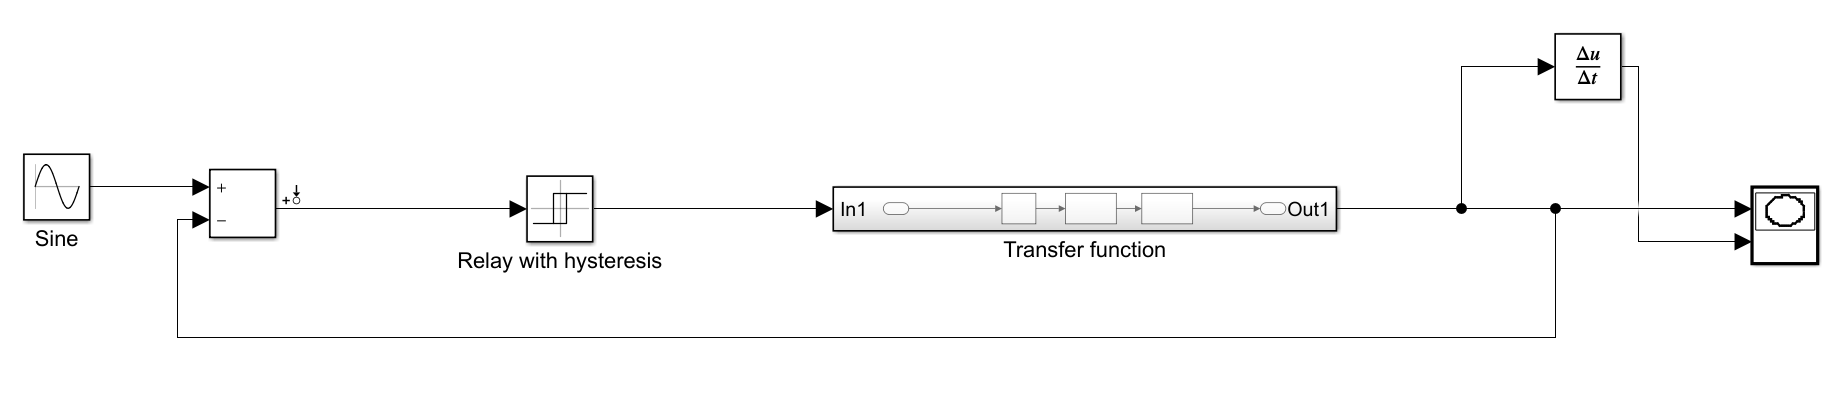
\includegraphics[width=\linewidth]{df_simulink.png}
	\caption{Non-linear system implementation in MATLAB Simulink.}
	\label{fig:df-simulink}
\end{figure}

\begin{figure}[h!]
	\centering
	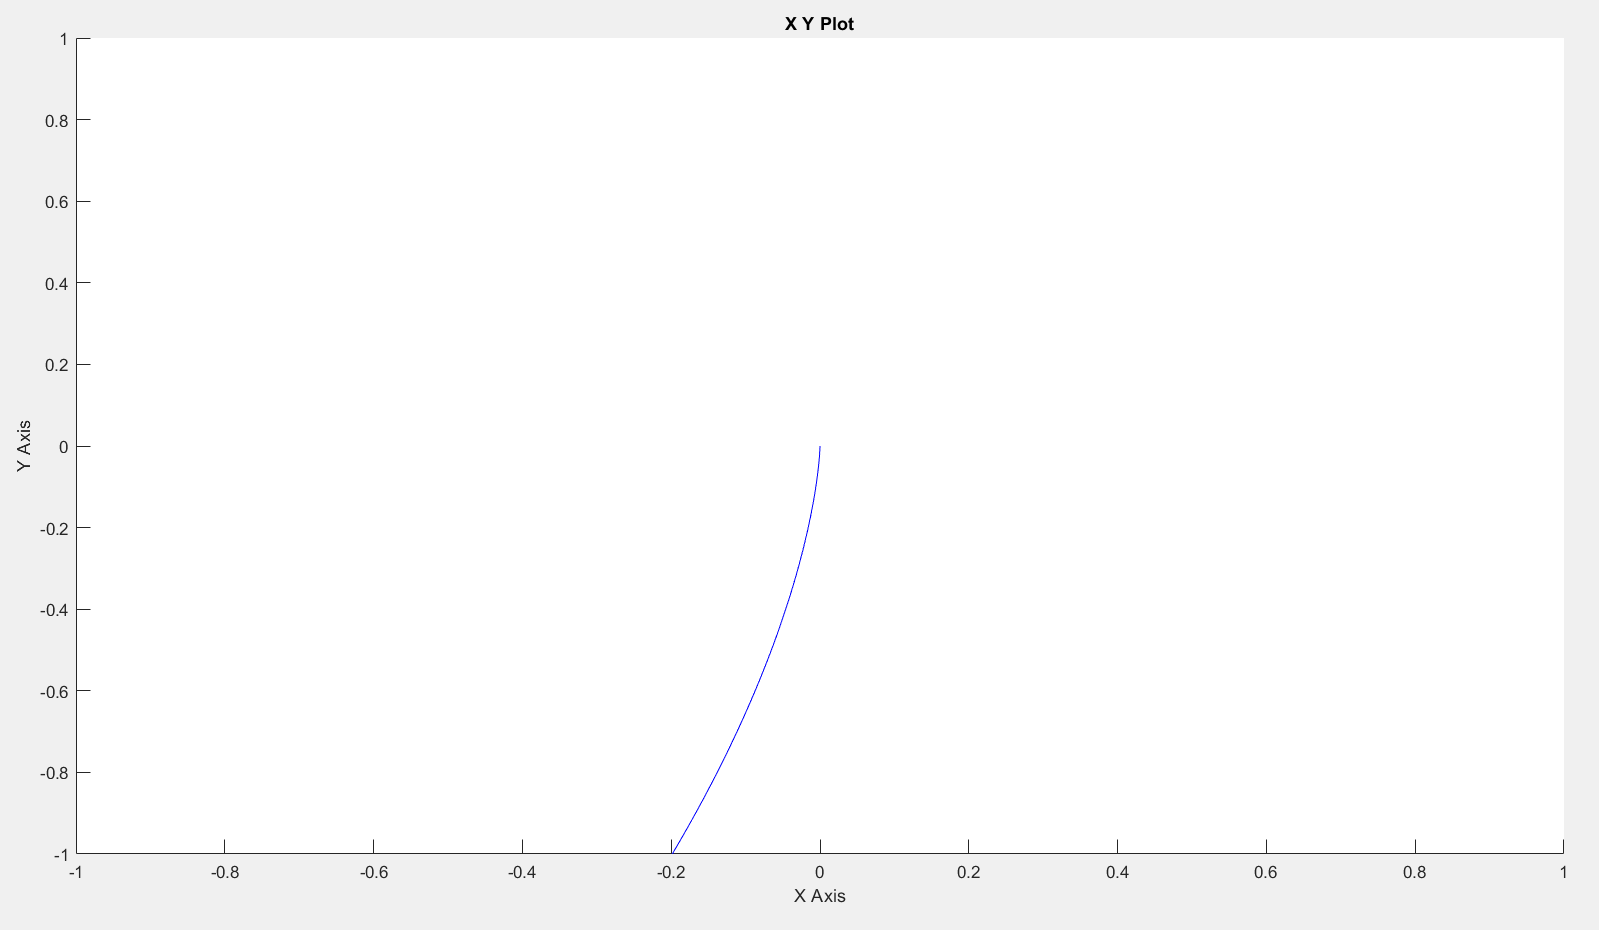
\includegraphics[width=0.9\linewidth]{LE3_df_phase.png}
	\caption{Phase plot of the system in Fig. \ref{fig:df-simulink}.}
	\label{fig:df-phase}
\end{figure}

\end{enumerate}

\end{document}